\documentclass[11pt]{article}
\usepackage[letterpaper,margin=0.78in]{geometry}
\usepackage[T1]{fontenc}
\usepackage{lmodern}
\usepackage{microtype}
\usepackage{amsmath,amssymb,amsthm,mathtools}
\usepackage{booktabs,longtable,array}
\usepackage{enumitem}
\usepackage{xcolor}
\usepackage{hyperref}
\usepackage{fancyhdr}
\usepackage{lastpage}
\usepackage{setspace}
\usepackage{graphicx}
\usepackage{url}
\usepackage{titlesec}
\usepackage{caption}
\usepackage{float}
\usepackage{verbatim}
\usepackage{tikz}
\usetikzlibrary{arrows.meta,positioning,shapes.multipart}

\definecolor{navy}{RGB}{25,56,95}
\definecolor{graybox}{RGB}{245,247,250}
\hypersetup{colorlinks=true,linkcolor=navy,citecolor=navy,urlcolor=navy,pdfauthor={Dr. Gregory C. Stamp},pdftitle={An Explicit Uniform Off-Diagonal Positivity Certificate in a Displacement Coordinate for a Binary Goldbach Circle-Method Specialization}}
\setstretch{1.00}
\setlength{\parindent}{1.2em}
\setlength{\parskip}{0.10em}
\setlist{nosep,leftmargin=1.6em}
\titleformat{\section}{\large\bfseries\color{navy}}{\thesection}{0.7em}{}
\titleformat{\subsection}{\normalsize\bfseries}{\thesubsection}{0.6em}{}
\pagestyle{fancy}
\fancyhf{}
\fancyhead[L]{\small Dr. G. C. Stamp -- Off-Diagonal Positivity Certificate}
\fancyhead[R]{\small Binary Goldbach Circle-Method Specialization}
\fancyfoot[C]{\small Page \thepage\ of \pageref{LastPage}}
\renewcommand{\headrulewidth}{0.3pt}

\newtheorem{theorem}{Theorem}[section]
\newtheorem{proposition}[theorem]{Proposition}
\newtheorem{lemma}[theorem]{Lemma}
\newtheorem{corollary}[theorem]{Corollary}
\theoremstyle{definition}
\newtheorem{definition}[theorem]{Definition}
\newtheorem{remark}[theorem]{Remark}

\newcommand{\e}{\mathrm{e}}
\newcommand{\Disp}{\mathrm{Disp}}
\newcommand{\RR}{Ramar\'{e}--Rumely}
\newcommand{\Delt}{\Delta}
\newcommand{\abs}[1]{\left|#1\right|}
\newcommand{\norm}[1]{\left\lVert#1\right\rVert}

\begin{document}

\begin{titlepage}
\centering
\vspace*{0.5in}
{\Large\bfseries\color{navy} An Explicit Uniform Off-Diagonal Positivity Certificate\\[0.15in]
 in a Displacement Coordinate for a Binary Goldbach Circle-Method Specialization\par}
\vspace{0.28in}
{\large Explicit prime-distribution estimates, rigorous interval computation,\\ and a Lean~4-verified structural bridge\par}
\vspace{0.45in}
{\Large Dr. Gregory C. Stamp\par}
\vspace{0.10in}
{\normalsize Independent Researcher\par}
\vspace{0.18in}
{\normalsize Revision v3.2 -- referee-response revision\par}
{\normalsize 10 September 2026\par}
\vfill
\end{titlepage}

\begin{abstract}
We establish an explicit positivity theorem for a fixed off-diagonal component arising from an exact displacement-coordinate reorganization of a Binary Goldbach circle-method specialization. Ordered prime pairs are grouped by their integer displacement from the target, preserving arithmetic and Fourier sign information that can be lost under premature absolute-value estimates. For the specialization studied here, the resulting off-diagonal contribution separates into three residue-class imbalances, and each is proved strictly positive for every even integer at least 56.

The proof combines exact analytic identities, explicit prime-distribution estimates of Ramar\'{e}--Rumely, rigorous Python-FLINT/Arb interval certification for the finite range, and Lean~4 verification of the structural bridge from signed-imbalance positivity to the intended core-domination inequality. A central fidelity result proves that the finite Stage-A lower certificate bounds the exact theorem object rather than a surrogate, and the treatment of prime jumps in the finite integral bound is matched directly to the generator code. The result closes this off-diagonal sign problem as a stable, reproducible module in a broader Binary Goldbach program. It does not prove the Binary Goldbach conjecture; an independent quantitative lower bound for the complementary major-side contribution remains the next mathematical gate.
\end{abstract}

\noindent\textbf{Keywords.} Binary Goldbach; circle method; Fourier transform; sinc kernel; primes in arithmetic progressions; rigorous computation; interval arithmetic; Lean 4; formal verification.

\section{Introduction and statement of contribution}

The Binary Goldbach conjecture asks whether every even integer $N>2$ is the sum of two primes. The modern analytic setting for additive prime problems begins with the Hardy--Littlewood circle method, where a Fourier coefficient of a prime exponential sum is decomposed into contributions from major and minor arcs. Hardy and Littlewood formulated the classical heuristic framework for the representation of integers by primes, and later treatments such as Vaughan's monograph systematized the major/minor-arc architecture and the associated exponential-sum estimates. The conjecture itself remains open, even though major advances in related additive-prime problems, including Helfgott's proof of the ternary Goldbach conjecture, demonstrate how explicit analytic estimates and rigorous finite verification can be combined successfully.

The purpose of this paper is substantially narrower. We do not attempt to close the full major/minor-arc inequality required for Binary Goldbach. Instead, we isolate a specific off-diagonal coordinate that arose from an exact decomposition of the major-arc kernel after preserving phase information long enough to expose cancellation by integer displacement. The principal object is a finite signed sum over
\[
k=p+q-N,
\]
where $p$ and $q$ range over the prime support relevant to the Fourier expansion. In this coordinate, the prime-log amplitude is nonnegative while the sign is carried by an explicit arithmetic factor and a centered Fourier kernel. The resulting problem is concrete: prove three strict signed inequalities, one in each residue class modulo $3$.

The specialization studied here is
\begin{equation}\label{eq:specialization}
P=K=3,\qquad Q=N/3,\qquad M=2.
\end{equation}
For these values, the arithmetic carrier collapses to a period-$6$ function and the Fourier kernel becomes an exact sinc profile. This makes it possible to connect: (i) the exact displacement decomposition; (ii) a sixth-root-of-unity filter; (iii) explicit estimates for primes in the reduced residue classes modulo $6$; (iv) a rigorous finite computation; and (v) a Lean proof of the structural implication that, conditional on positivity of the signed imbalance, full support saturation yields the intended off-diagonal core-domination certificate. Lean does not verify the external analytic or Arb positivity premise.

The contribution should be read as an explicit theorem about a specialized off-diagonal object, not as a novelty claim for the individual analytic tools. Root-of-unity filters, sinc/Fourier kernels, explicit prime-number-theorem estimates in arithmetic progressions, and interval arithmetic are standard. The contribution is the exact assembly of these ingredients around the displacement coordinate and the uniform closure of the resulting certificate above the stated threshold with both reproducibility and a formal structural bridge.


\subsection{Meaning of the off-diagonal positivity certificate}\label{sec:meaning}

The phrase \emph{off-diagonal positivity certificate} has a precise meaning in this paper. The displacement $k=0$ is the representation fiber $p+q=N$ itself. The off-diagonal object is obtained by removing that fiber and retaining every populated displacement with $k\ne0$. This removal is essential: the theorem does not assume, encode, or infer the existence of a Goldbach representation from the $k=0$ term.

For each residue class modulo $3$, the remaining displacement terms carry both a nonnegative prime-log amplitude and an explicit sign determined by the arithmetic carrier and centered Fourier kernel. Their signed sum is $\Delta_r(N)=P_r-N_r$, where $P_r$ is the total favorable mass and $N_r$ is the total unfavorable magnitude. Thus $\Delta_r(N)>0$ means that, after the exact arithmetic and Fourier weights are applied, the favorable off-diagonal contribution strictly dominates the unfavorable contribution in that residue class. Because every populated displacement lies in the intrinsic window $|k|<N$, the favorable core is the entire positive mass, so positivity is exactly equivalent to the core-domination inequality $N_r<C_2(r)=P_r$.

This certificate is needed because the off-diagonal terms form a signed correction inside the larger circle-method architecture. Without such control, the off-diagonal term cannot be combined safely with a positive major-side contribution in the larger quantitative inequality. Theorem~\ref{thm:main} removes that uncertainty for the fixed specialization studied here. What it does \emph{not} do is supply the independent positive lower bound on the complementary major-side quantity required to complete the full Binary Goldbach argument.

\subsection{Contributions and mathematical significance}\label{sec:significance-intro}

Theorem~\ref{thm:main} settles a precisely defined sign question for the fixed displacement-coordinate specialization studied here. It does not resolve Binary Goldbach or the classical minor-arc/first-moment barrier. Rather, it proves that the favorable weighted off-diagonal mass dominates the unfavorable weighted mass in each residue class for every even target covered by the theorem. Five features organize the contribution.

\begin{enumerate}
\item \textbf{Exact displacement reorganization.} The passage from ordered prime pairs $(p,q)$ to $k=p+q-N$ is not an approximation. It aggregates the nonnegative prime-log amplitude on each fiber while retaining the arithmetic carrier and Fourier sign as explicit functions of a single integer. This prevents the cancellation information from being erased prematurely by absolute values.
\item \textbf{A fixed arithmetic geometry.} For $P=K=3$, the carrier becomes a six-periodic law and is strictly positive on the three even bulk classes associated with the mod-$3$ residue coordinates. Together with the sinc kernel, this turns a diffuse phase problem into three concrete signed inequalities.
\item \textbf{Uniform closure above the threshold.} The proof is not merely asymptotic and not merely computational. A finite rigorous certificate, a square-root explicit prime-distribution regime, and a relative-error regime overlap to cover every even $N\ge56$ with no transition gap.
\item \textbf{Object fidelity as a theorem.} The finite Stage-A quantity is proved to be a lower bound for the exact $\Delta_r(N)$ itself. This closes the central computer-assisted-proof failure mode in which a rigorous computation certifies a nearby surrogate rather than the mathematical object stated in the theorem.
\item \textbf{Hybrid verification with separated epistemic burdens.} Analytic derivation, interval-arithmetic positivity, independent artifact-integrity checking, and Lean structural formalization are treated as distinct verification layers. No layer is claimed to certify work that it does not actually perform.
\end{enumerate}

The methodological comparison with Helfgott's ternary Goldbach work is one of \emph{proof discipline}, not theorem strength or technical identity. Helfgott's proof combines explicit circle-method estimates with rigorous finite verification and carefully controlled computational inputs \cite{HelfgottMajor2013,HelfgottPlatt2013,Helfgott2015}. The present theorem applies a similar standard of explicitness to a much narrower Binary-Goldbach-derived off-diagonal object. The individual ingredients used here are classical; the potentially nonstandard contribution is their exact assembly around the displacement coordinate and the reproducible closure of that specific positivity theorem. A definitive priority or ``first use'' claim is intentionally not made without a dedicated literature review.

\begin{figure}[H]
\centering
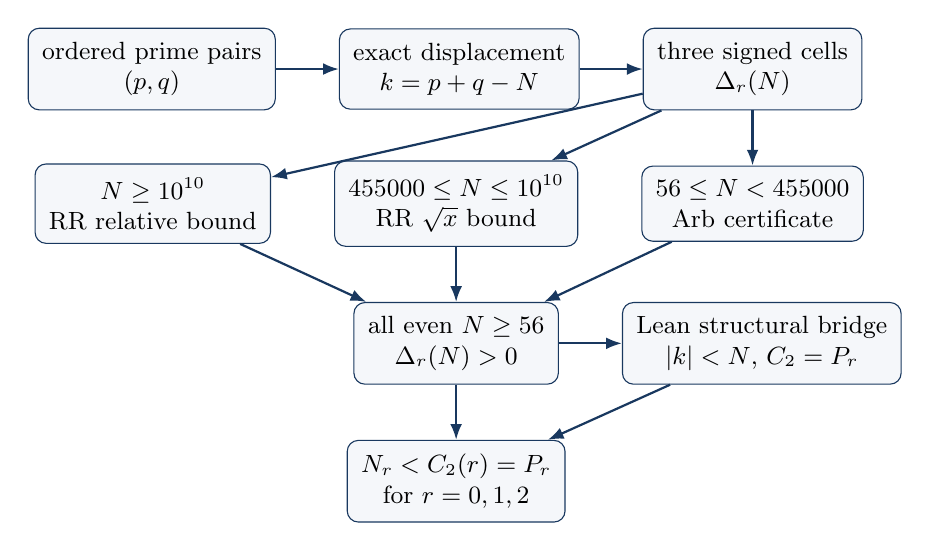
\begin{tikzpicture}[
  node distance=7mm and 8mm,
  box/.style={draw=navy, rounded corners, align=center, inner sep=5pt, fill=graybox, font=\small},
  arr/.style={-{Latex[length=2mm]}, thick, draw=navy}
]
\node[box] (pairs) {ordered prime pairs\\$(p,q)$};
\node[box, right=of pairs] (disp) {exact displacement\\$k=p+q-N$};
\node[box, right=of disp] (res) {three signed cells\\$\Delta_r(N)$};
\node[box, below=of res] (finite) {$56\le N<455000$\\Arb certificate};
\node[box, left=of finite] (sqrt) {$455000\le N\le10^{10}$\\RR $\sqrt{x}$ bound};
\node[box, left=of sqrt] (large) {$N\ge10^{10}$\\RR relative bound};
\node[box, below=of sqrt] (alln) {all even $N\ge56$\\$\Delta_r(N)>0$};
\node[box, right=of alln] (lean) {Lean structural bridge\\$|k|<N$, $C_2=P_r$};
\node[box, below=of alln] (cert) {$N_r<C_2(r)=P_r$\\for $r=0,1,2$};
\draw[arr] (pairs)--(disp); \draw[arr] (disp)--(res);
\draw[arr] (res)--(finite); \draw[arr] (res)--(sqrt); \draw[arr] (res)--(large);
\draw[arr] (finite)--(alln); \draw[arr] (sqrt)--(alln); \draw[arr] (large)--(alln);
\draw[arr] (alln)--(lean); \draw[arr] (lean)--(cert); \draw[arr] (alln)--(cert);
\end{tikzpicture}
\caption{Proof-navigation architecture. The analytic/computational branch proves positivity of the exact signed displacement imbalances; the Lean branch verifies the structural implication from that positivity to the intrinsic-core inequality.}
\label{fig:architecture}
\end{figure}

\subsection{Main theorem}

The definitions needed to state the result self-containedly are introduced in Sections~\ref{sec:structure}--\ref{sec:residue}. For the moment, let $\Delta_r(N)$ denote the exact signed displacement imbalance in residue $r\pmod3$, and let $P_r$ and $N_r$ denote its total positive and total negative-magnitude masses. Let $C_2(r)$ be the positive mass restricted to the intrinsic lobe-pair window $\abs{k}<3Q=N$.

\begin{theorem}[Explicit off-diagonal certificate]\label{thm:main}
For the specialization \eqref{eq:specialization}, every even integer $N\ge56$ satisfies
\[
\Delta_0(N)>0,\qquad \Delta_1(N)>0,\qquad \Delta_2(N)>0.
\]
Moreover every populated displacement satisfies $\abs{k}<N$, so $C_2(r)=P_r$. Consequently,
\[
\boxed{\;N_r<C_2(r)=P_r,\qquad r=0,1,2.\;}
\]
\end{theorem}

The proof is partitioned into the three ranges
\[
56\le N\le454998,\qquad
455000\le N\le10^{10},\qquad
N\ge10^{10}.
\]
The first is certified by rigorous ball arithmetic, the second by an explicit $\sqrt{N}$ error estimate, and the third by a linear relative-error estimate. The two analytic regimes meet at the closed endpoint $10^{10}$, which belongs to both stated ranges, while the finite certificate ends at $454998$, the immediately preceding even integer before $455000$. Hence there is no uncovered even target.

\subsection{Relation to classical literature}

The circle method and the decomposition of additive prime problems into structured and oscillatory pieces are classical; see Hardy--Littlewood and Vaughan. Sieve-theoretic structure and Ramanujan-sum manipulations are treated systematically by Friedlander and Iwaniec, while Montgomery and Vaughan give a modern account of additive prime number theory and large-sieve methods. The load-bearing explicit arithmetic-progression input here is the 1996 paper of \RR. Section~5.2, Theorem~5.2.1 (printed p.~421) gives the pointwise square-root estimate through $10^{10}$ for every modulus in Table~1. Theorem~1 together with Table~1 (printed p.~419) gives explicit relative errors for $x\ge x_0$; the table states that its reported values are rounded upward in the last decimal place. In particular, the row $k=6$, $x_0=10^{10}$ gives $\epsilon=0.002238$ \cite{RamareRumely1996}. Later work of Bennett, Martin, O'Bryant and Rechnitzer extends explicit bounds for primes in arithmetic progressions much further; we retain the older \RR\ constants because they match the fixed modulus and the proof architecture used in the computational certificate.

Helfgott's ternary Goldbach work is relevant methodologically rather than as a direct input. His major-arc analysis explicitly incorporates rigorous finite verification of analytic inputs, while the completed ternary proof combines explicit circle-method estimates with a very large numerical verification range \cite{HelfgottMajor2013,HelfgottPlatt2013,Helfgott2015}. The present paper follows a related epistemic discipline at a much smaller and more localized scale: exact formulas first, explicit error accounting second, rigorous finite computation third, independent artifact checking fourth, and formal structural verification last. No claim is made that the present theorem is comparable in scope to the ternary Goldbach theorem.

\section{Exact displacement structure}\label{sec:structure}

Let
\[
\mathcal P_N=\{p\le N: p\text{ prime}\}
\]
and define the ordered prime-support pair set $\mathcal P_N\times\mathcal P_N$. For an ordered pair $(p,q)$ define the integer displacement
\begin{equation}\label{eq:disp}
k=p+q-N\in\mathbb Z.
\end{equation}
The set of populated displacements is
\[
\Disp(N)=\{p+q-N:(p,q)\in\mathcal P_N^2\}.
\]
The exact prime-log fiber mass at displacement $k$ is
\begin{equation}\label{eq:amplitude}
A_N(k)=
\sum_{\substack{p,q\le N\;\mathrm{prime}\\p+q-N=k}}
(\log p)(\log q).
\end{equation}
For the off-diagonal coordinate we remove $k=0$ by setting $A_N^{\mathrm{off}}(0)=0$ and $A_N^{\mathrm{off}}(k)=A_N(k)$ for $k\ne0$. The exact structured major-arc off-diagonal object in the underlying formal development is a finite sum
\begin{equation}\label{eq:exact-offdiag}
\mathrm{OffDiag}(N)
=
\sum_{k\in\Disp(N)}
A_N^{\mathrm{off}}(k)\,\mathcal K_N(k),
\end{equation}
where the kernel $\mathcal K_N(k)$ factors into an arithmetic carrier and a centered Fourier base kernel. Equation \eqref{eq:exact-offdiag} is an identity, not an estimate; this exactness is essential because all later cancellation occurs between populated displacements rather than between artificial surrogate terms.

For the fixed specialization \eqref{eq:specialization}, the arithmetic factor is especially simple. Define
\[
R_{3,3}(k)=
\sum_{\substack{d\in\{1,2,3\}\\d\mid\abs{k}}}dM_{3,3}(d),
\]
with
\[
M_{3,3}(1)=-1,\qquad M_{3,3}(2)=1,\qquad M_{3,3}(3)=1.
\]
Therefore
\begin{equation}\label{eq:carrier}
\boxed{
R_{3,3}(k)=-1+2\mathbf1_{2\mid k}+3\mathbf1_{3\mid k}.
}
\end{equation}
On the six residue classes modulo $6$ this is
\begin{center}
\begin{tabular}{c|rrrrrr}
$k\bmod6$&0&1&2&3&4&5\\\hline
$R_{3,3}(k)$&4&-1&1&2&1&-1
\end{tabular}
\end{center}
The kernel sign is thus encoded by a finite periodic law.

\section{The centered sinc kernel and residue coordinates}\label{sec:residue}

The centered major-arc base kernel at scale $Q$ is the Fourier transform of the centered interval $[-1/Q,1/Q]$. With the convention $e(x)=\exp(2\pi i x)$,
\begin{equation}\label{eq:sinc-general}
B_Q(k)
=\int_{-1/Q}^{1/Q}e(k\beta)\,d\beta
=\begin{cases}
\dfrac{\sin(2\pi k/Q)}{\pi k},&k\ne0,\\[2mm]
\dfrac2Q,&k=0.
\end{cases}
\end{equation}
For $Q=N/3$,
\begin{equation}\label{eq:sinc}
B_{N/3}(k)=
\begin{cases}
\dfrac{\sin(6\pi k/N)}{\pi k},&k\ne0,\\[2mm]
\dfrac6N,&k=0.
\end{cases}
\end{equation}
This identity gives a useful geometric interpretation: the same parameter $Q$ that sets the major-arc frequency width also fixes the zero spacing and lobe scale in displacement space. The interpretation is expository; no wavelet or frame theorem is used in the proof.

Define the signed displacement term
\begin{equation}\label{eq:T}
T_N(k)=A_N^{\mathrm{off}}(k)R_{3,3}(k)B_{N/3}(k).
\end{equation}
For $r\in\{0,1,2\}$ define
\begin{equation}\label{eq:delta}
\Delta_r(N)
=
\sum_{\substack{k\in\Disp(N)\\k\equiv r\;(3)}}T_N(k).
\end{equation}
Let
\[
P_r=
\sum_{\substack{k\in\Disp(N)\\k\equiv r\;(3)}}\max(T_N(k),0),
\quad
N_r=
\sum_{\substack{k\in\Disp(N)\\k\equiv r\;(3)}}\max(-T_N(k),0).
\]
Then, exactly,
\begin{equation}\label{eq:PN}
\Delta_r=P_r-N_r.
\end{equation}
The intrinsic favorable core with $M=2$ is the same positive part restricted to
\[
\abs{k}<(M+1)Q=3(N/3)=N.
\]
We denote this restricted positive mass by $C_2(r)$.

\begin{lemma}[Full support lies in the $M=2$ window]\label{lem:window}
If $N\ge4$ is even and $k\in\Disp(N)$, then $\abs{k}<N$.
\end{lemma}
\begin{proof}
Write $k=p+q-N$ with $p,q\le N$ prime. Since $N\ge4$ is even, $N$ is not prime; hence $p,q<N$. Also $p,q\ge2$. Therefore
\[
4-N\le p+q-N\le2(N-1)-N=N-2.
\]
Both endpoints lie strictly between $-N$ and $N$, proving the claim.
\end{proof}

The same argument is formalized in Lean in Section~\ref{sec:lean}. Lemma~\ref{lem:window} implies
\begin{equation}\label{eq:coreeq}
\boxed{C_2(r)=P_r.}
\end{equation}
Combining \eqref{eq:PN} and \eqref{eq:coreeq} gives the structural equivalence
\begin{equation}\label{eq:structural-equiv}
\boxed{
\Delta_r>0
\iff P_r>N_r
\iff N_r<C_2(r).
}
\end{equation}
Thus the analytic task reduces exactly to proving three strict positive imbalances.

\section{Bulk reduction modulo 6 and the sixth-root filter}\label{sec:rootfilter}

Consider first the bulk sector $p,q>3$. Both primes are odd, while $N$ is even, so the displacement $k=p+q-N$ is even. Consequently,
\[
\begin{array}{ccl}
r=0&\Longrightarrow&k\equiv0\pmod6,\\
r=1&\Longrightarrow&k\equiv4\pmod6,\\
r=2&\Longrightarrow&k\equiv2\pmod6.
\end{array}
\]
From \eqref{eq:carrier}, the carrier values in these three bulk classes are $4,1,1$, respectively. In particular, the bulk carrier is strictly positive in all three residue coordinates.

Define the reduced-prime exponential sum
\begin{equation}\label{eq:S6}
S_6(\alpha)=
\sum_{\substack{p\le N\\p>3}}
(\log p)e(p\alpha).
\end{equation}
For $a\in\{0,4,2\}$, define the unweighted bulk sinc sum
\begin{equation}\label{eq:Dtilde}
\widetilde D_a(N)
=
\sum_{\substack{p,q>3\\p,q\le N\\p+q-N\equiv a\;(6)}}
(\log p)(\log q)B_{N/3}(p+q-N).
\end{equation}
The sixth-root filter is the identity
\[
\mathbf1_{m\equiv0\;(6)}
=\frac16\sum_{j=0}^5 e(mj/6).
\]
Using the integral representation
\[
B_{N/3}(p+q-N)
=
\int_{-3/N}^{3/N}e((p+q-N)\beta)\,d\beta,
\]
we obtain the exact formula
\begin{equation}\label{eq:root-filter}
\boxed{
\widetilde D_a(N)
=
\frac16\sum_{j=0}^{5}
 e\!\left(-\frac{(N+a)j}{6}\right)
\int_{-3/N}^{3/N}
 e(-N\beta)
 S_6\!\left(\beta+\frac j6\right)^2d\beta.
}
\end{equation}
No inequality has yet been used. Throughout this manuscript pair sums are \emph{ordered}: $(p,q)$ and $(q,p)$ are distinct when $p
e q$, while $p=q$ contributes once. The phase $N+a$ is explicit, and the zero displacement remains visible until it is subtracted in Section~\ref{sec:exceptions}.

\section{Explicit prime-distribution input through $10^{10}$}\label{sec:finiteanalytic}

For $h\in\{1,5\}$ write
\[
\theta(x;6,h)=\sum_{\substack{p\le x\\p\equiv h\;(6)}}\log p
=\frac{x}{2}+E_h(x).
\]
The load-bearing finite-source input is \RR, Section~5.2, Theorem~5.2.1 (printed p.~421). For every modulus in their Table~1, uniformly over $0\le x\le10^{10}$,
\begin{equation}\label{eq:RRsqrt}
\boxed{\abs{\theta(x;6,h)-x/2}\le2.072\sqrt{x}.}
\end{equation}
Thus the bound used inside the partial-summation integral is pointwise in its integration variable. The theorem applies to $k=6$ because $6$ is one of the moduli in Table~1 \cite{RamareRumely1996}. The later paper of Bennett--Martin--O'Bryant--Rechnitzer extends explicit prime-distribution bounds substantially, but \eqref{eq:RRsqrt} is retained here because the proof architecture was constructed around it.

\medskip
\noindent\textbf{Primary-source lock.} The numerical constant $2.072$ is not inferred from a secondary citation. In the original Ramar\'{e}--Rumely paper, Theorem~5.2.1 on printed p.~421 states the bound uniformly for \emph{all} moduli in Table~1 over $0\le x\le10^{10}$. Since $k=6$ appears explicitly in Table~1, the modulus-$6$ use above is source-locked. This point matters because the lower-end margin at $N=455000$ is small relative to the scale of the square-root error term.


Let
\[
V_N(\beta)=\int_0^N e(\beta x)\,dx,
\qquad
c_j=\frac12\left(e(j/6)+e(5j/6)\right)=\cos(\pi j/3).
\]
By Stieltjes partial summation over the two reduced classes modulo $6$,
\begin{equation}\label{eq:approxS}
S_6\!\left(\beta+\frac j6\right)
=c_jV_N(\beta)+\eta_j(\beta).
\end{equation}
We now record the uniform error constant explicitly.

\begin{lemma}[Finite-source partial-summation error]\label{lem:D}
For $\abs{\beta}\le3/N$ and $N\le10^{10}$,
\[
\abs{\eta_j(\beta)}\le D\sqrt N,
\]
where
\begin{equation}\label{eq:D}
\boxed{
D=2(2.072)(1+4\pi)
=56.2190398259044127207567767\ldots.
}
\end{equation}
\end{lemma}
\begin{proof}
For a single residue class, the endpoint contribution is at most $2.072\sqrt N$. The integral term in partial summation contains $2\pi\abs{\beta}\int_0^N\abs{E_h(t)}dt$. Using \eqref{eq:RRsqrt},
\[
\int_0^N2.072\sqrt t\,dt
=2.072\cdot\frac23N^{3/2}.
\]
Since $\abs{\beta}\le3/N$, the integral contribution is bounded by
\[
2\pi\frac3N\cdot2.072\frac23N^{3/2}
=2.072\,(4\pi)\sqrt N.
\]
Thus one residue class contributes at most $2.072(1+4\pi)\sqrt N$. There are two reduced classes, $1$ and $5$ modulo $6$, giving \eqref{eq:D}.
\end{proof}

The exact $L^1$ norm of the model integral on the short frequency window is
\begin{equation}\label{eq:L}
\begin{split}
L&=\int_{-3/N}^{3/N}\abs{V_N(\beta)}\,d\beta\\
&=\frac2\pi\int_0^3\frac{\abs{\sin(\pi t)}}{t}\,dt\\
&=1.61849929702031725197023676\ldots.
\end{split}
\end{equation}
The scaling is independent of $N$. Since $c_j=(1,1/2,-1/2,-1,-1/2,1/2)$ up to order, we have
\begin{equation}\label{eq:cjabs}
\sum_{j=0}^5\abs{c_j}=4.
\end{equation}

Substituting \eqref{eq:approxS} into \eqref{eq:root-filter}, expanding the square, and applying \eqref{eq:cjabs} gives the following common bulk estimate.

\begin{proposition}[Bulk approximation]\label{prop:bulk}
For $a\in\{0,2,4\}$ and $N\le10^{10}$,
\begin{equation}\label{eq:bulk-bound}
\boxed{
\abs{\widetilde D_a(N)-\rho_{N+a}HN}
\le\frac43LD\sqrt N+6D^2.
}
\end{equation}
Numerically,
\begin{equation}\label{eq:AB}
\frac43LD
=121.3206352498446810338805013\ldots,
\end{equation}
\begin{equation}
6D^2
=18963.48263367975876095244979\ldots.
\end{equation}
\end{proposition}
\begin{proof}
The cross term has absolute value at most
\[
\frac16\sum_{j=0}^5
2\abs{c_j}D\sqrt N
\int_{-3/N}^{3/N}\abs{V_N(\beta)}d\beta
=\frac13D\sqrt N\,L\sum_j\abs{c_j},
\]
which is $(4/3)LD\sqrt N$. For the quadratic term, $\abs{\eta_j}^2\le D^2N$ and the integration interval has length $6/N$, so each $j$ contributes at most $6D^2$ before the outer factor $1/6$. Summing six $j$ values leaves $6D^2$.
\end{proof}

\section{The main Fourier coefficient and singular integral}\label{sec:maincoefficient}

Define the discrete Fourier coefficient
\begin{equation}\label{eq:rho}
\rho_s
=\frac16\sum_{j=0}^5c_j^2e(-sj/6).
\end{equation}
Direct evaluation gives
\begin{equation}\label{eq:rho-values}
\rho_s=
\begin{cases}
1/2,&s\equiv0\pmod6,\\
1/4,&s\equiv2,4\pmod6,\\
0,&s\text{ odd}.
\end{cases}
\end{equation}
Because $N$ and $a$ are even, $N+a$ is even, so
\begin{equation}\label{eq:rho-lower}
\rho_{N+a}\ge\frac14.
\end{equation}

The model integral in \eqref{eq:bulk-bound} is obtained by scaling $t=N\beta$:
\[
\int_{-3/N}^{3/N}
e(-N\beta)V_N(\beta)^2d\beta
=HN,
\]
where
\begin{equation}\label{eq:H}
H
=\int_{-3}^{3}e(-t)
\left(\int_0^1e(tu)du\right)^2dt
=\frac2\pi\operatorname{Si}(6\pi).
\end{equation}
Using $\operatorname{Si}(x)=\pi/2-\int_x^\infty\sin u/u\,du$ and one integration by parts,
\[
\abs{\int_x^\infty\frac{\sin u}{u}du}\le\frac2x.
\]
At $x=6\pi$ this yields
\begin{equation}\label{eq:Hlower}
\boxed{
H\ge H_{\mathrm{low}}
:=1-\frac2{3\pi^2}
=0.932452544238441485704080358\ldots.
}
\end{equation}
Combining \eqref{eq:rho-lower} and \eqref{eq:Hlower}, the weakest main coefficient common to all three residues is
\begin{equation}\label{eq:c0}
\boxed{
c_0:=\frac14H_{\mathrm{low}}
=0.233113136059610371426020089\ldots.
}
\end{equation}
The $r=0$ bulk carrier is $4$. This does not mean that only the main term is multiplied by $4$; the corresponding bulk error is multiplied by $4$ as well. Section~\ref{sec:exceptions} records the explicit accounting showing that the common condition $F(N)>0$ remains sufficient for $r=0$.

\section{Exceptional small primes, zero displacement, and the cutoff}\label{sec:exceptions}

The bulk analysis excluded pairs involving $2$ or $3$ and temporarily retained the zero displacement in the root-filtered $a=0$ sum. Both effects can be bounded explicitly.

From \eqref{eq:sinc},
\begin{equation}\label{eq:Bbound}
\abs{B_{N/3}(k)}\le\frac6N,
\end{equation}
and from \eqref{eq:carrier},
\begin{equation}\label{eq:Rbound}
\abs{R_{3,3}(k)}\le4.
\end{equation}
A safe common estimate for all ordered pairs containing at least one prime in $\{2,3\}$ is
\begin{equation}\label{eq:small}
\boxed{
\abs{E_{\mathrm{small}}(N)}
\le48\log6\,\log N.
}
\end{equation}
The bound deliberately overcounts; overcounting is harmless because it is subtracted as an error budget.

For $r=0$, the root-filtered bulk includes $k=0$ while the off-diagonal amplitude deletes it. The carrier at $0$ is $4$ and $B_{N/3}(0)=6/N$, so the deleted carrier-weighted term is
\[
\frac{24}{N}A_N(0).
\]
Without assuming the existence of any Goldbach representation, we have the trivial estimate
\[
A_N(0)
\le N(\log N)^2,
\]
which yields
\begin{equation}\label{eq:diag}
\boxed{
E_{\mathrm{diag}}(N)
\le24(\log N)^2.
}
\end{equation}
This deletion is therefore non-circular.

Let
\[
E_{\rm bulk}(N)=A\sqrt N+B,
\qquad
E_s(N)=48\log6\,\log N,
\qquad
E_d(N)=24(\log N)^2.
\]
For $r=1,2$ the carrier is $1$, so
\[
\Delta_r\ge c_0N-E_{\rm bulk}-E_s
\ge c_0N-E_{\rm bulk}-E_s-E_d.
\]
For $r=0$ the carrier is $4$ and the diagonal deletion applies, hence
\begin{align}
\Delta_0
&\ge4(c_0N-E_{\rm bulk})-E_d-E_s\\
&=4\bigl(c_0N-E_{\rm bulk}-E_d-E_s\bigr)+3E_d+3E_s.\label{eq:r0-accounting}
\end{align}
Therefore the same sufficient condition $F(N)>0$ proves positivity in all three residues; equation~\eqref{eq:r0-accounting} is the explicit $r=0$ accounting.

A common sufficient lower bound for all three residue imbalances is
\begin{equation}\label{eq:F}
F(N)
=c_0N
-A\sqrt N
-B
-24(\log N)^2
-48\log6\,\log N,
\end{equation}
where
\[
A=121.3206352498446810338805013\ldots,
\quad
B=18963.48263367975876095244979\ldots.
\]
A high-precision recomputation gives a unique crossing
\begin{equation}\label{eq:Froot}
N_*
=454479.093587170978288654443\ldots.
\end{equation}
At the clean integer threshold,
\begin{equation}\label{eq:F455}
\boxed{
F(455000)
=73.75737924545603871534874\ldots>0.
}
\end{equation}
Moreover
\begin{equation}\label{eq:Fprime}
F'(x)
=c_0-\frac{A}{2\sqrt x}
-\frac{48\log x}{x}
-\frac{48\log6}{x},
\end{equation}
and
\begin{equation}\label{eq:F2}
F''(x)
=\frac{A}{4x^{3/2}}
+\frac{48(\log x-1+\log6)}{x^2}>0
\qquad(x\ge455000).
\end{equation}
Finally,
\begin{equation}\label{eq:Fp455}
F'(455000)
=0.1416208893276761769268907\ldots>0.
\end{equation}
For publication these decimal evaluations are not trusted as floating-point facts. The companion script \texttt{certify\_publication\_bounds\_rational.py} uses exact rational arithmetic: Machin's formula with alternating rational series encloses $\pi$; alternating rational series plus a Lipschitz correction enclose the required sine integrals; logarithms are enclosed through the $\operatorname{atanh}$ series after power-of-two range reduction; and square roots are enclosed by integer square roots. It independently certifies
\begin{equation}\label{eq:Finterval}
\boxed{F(455000)\in[73.757379245456,\,73.757379245457]}
\end{equation}
and
\begin{equation}\label{eq:Fpinterval}
\boxed{F'(455000)\in[0.141620889327676,\,0.141620889327677].}
\end{equation}
The exact crossing $N_*$ in \eqref{eq:Froot} is therefore descriptive rather than load-bearing. Since $F''(x)>0$ on the stated range, \eqref{eq:Finterval}--\eqref{eq:Fpinterval} prove that $F$ is strictly increasing on $[455000,10^{10}]$, and we obtain
\begin{equation}\label{eq:finiteanalytic-positive}
\Delta_r(N)>0
\qquad(r=0,1,2)
\end{equation}
for every even $455000\le N\le10^{10}$.

\section{Explicit continuation for $N\ge10^{10}$}\label{sec:largeN}

The large-$N$ regime uses \RR's Theorem~1 and Table~1 (printed p.~419). Table~1 reports
\[
\epsilon=\max\bigl(\epsilon(\theta,x_0,k),\epsilon(\psi,x_0,k)\bigr)
\]
and states that the entries are rounded upward in the last decimal place. In the row $k=6$ and column $x_0=10^{10}$ it gives
\begin{equation}\label{eq:epsilon}
\boxed{\epsilon=0.002238.}
\end{equation}
This value has been checked directly against the primary-source Table~1 on printed p.~419. Since $\varphi(6)=2$, the normalization used below is therefore
\[
\epsilon/\varphi(6)=0.002238/2=0.001119.
\]
Under their normalization \cite{RamareRumely1996},
\[
\max_{1\le y\le x}
\abs{\theta(y;6,h)-y/2}
\le\epsilon\frac{x}{\varphi(6)}
=0.001119x,
\qquad x\ge10^{10}.
\]
Set
\begin{equation}\label{eq:delta-large}
\delta=0.001119.
\end{equation}
For the conservative publication estimate, apply the maximal bound directly in partial summation. For one reduced residue class,
\[
\abs{E_h(N)}+2\pi\abs{\beta}\int_0^N\abs{E_h(t)}dt
\le\delta N+2\pi\frac3N(\delta N)N
=\delta N(1+6\pi).
\]
Accounting for both residue classes gives
\begin{equation}\label{eq:dinf}
\boxed{
d_\infty
=2\delta(1+6\pi)
=0.0444233061524037436060763754\ldots.
}
\end{equation}
The same expansion as in Proposition~\ref{prop:bulk} yields the bulk error coefficient
\begin{equation}\label{eq:einf}
\boxed{
e_\infty
=\frac43Ld_\infty+6d_\infty^2
=0.107706033815706211647196984\ldots.
}
\end{equation}
Thus the linear coefficient margin is
\begin{equation}\label{eq:minf}
\boxed{
m_\infty:=c_0-e_\infty
=0.125407102243904159778823106\ldots>0.
}
\end{equation}

To avoid the vague phrase ``for all sufficiently large $N$,'' define
\begin{equation}\label{eq:G}
G(N)
=m_\infty N
-24(\log N)^2
-48\log6\,\log N.
\end{equation}
Direct evaluation at the exact transition point gives
\begin{equation}\label{eq:G1e10}
\boxed{
G(10^{10})
=1254056317.557827293420385\ldots>0.
}
\end{equation}
Moreover
\[
G'(x)=m_\infty-\frac{48(\log x+\log6)}{x}
\]
and
\[
G''(x)=\frac{48(\log x+\log6-1)}{x^2}>0
\qquad(x\ge10^{10}).
\]
At the boundary,
\begin{equation}\label{eq:Gp1e10}
\boxed{
G'(10^{10})
=0.1254069831193742437699663\ldots>0.
}
\end{equation}
The same independent rational interval script certifies
\begin{align}
G(10^{10})&\in[1254056317.557827,\,1254056317.557828],\label{eq:Ginterval}\\
G'(10^{10})&\in[0.125406983119374,\,0.125406983119375],\label{eq:Gpinterval}\\
m_\infty&\in[0.125407102243904159,\,0.125407102243904160].\label{eq:minfinterval}
\end{align}
Hence $G$ is strictly increasing for every $x\ge10^{10}$, proving \eqref{eq:finiteanalytic-positive} for all even $N\ge10^{10}$. Because the finite-source regime already includes $N=10^{10}$, there is no transition gap.

\section{Rigorous finite certification below $455000$}\label{sec:finitecert}

The remaining even interval is
\[
56\le N<455000,
\]
which contains exactly
\[
\frac{454998-56}{2}+1=227472
\]
targets. A rigorous notebook using Python-FLINT/Arb at $160$ bits was executed locally. Arb represents real quantities by midpoint-radius balls and propagates rigorous enclosures, so a positive lower endpoint is a mathematical certificate of positivity provided the implementation computes the intended expression.

The finite computation was deliberately separated into two stages.

\subsection{Stage A: sharpened analytic Arb sweep with exact prime data}

Stage A does \emph{not} apply the coarse uniform function $F(N)$ from Section~\ref{sec:exceptions}. Instead it keeps the actual finite prime-distribution error at each target. For $h\in\{1,5\}$ define
\begin{equation}\label{eq:AhJh}
A_h(N)=\abs{E_h(N)},\qquad
J_h(N)=\int_0^N\abs{E_h(x)}\,dx.
\end{equation}
Partial summation gives the target-specific pointwise bound
\begin{equation}\label{eq:etaAJ}
\abs{\eta_h(\beta)}\le A_h+2\pi\abs{\beta}J_h.
\end{equation}
Instead of maximizing $\abs{\beta}$ before integration, the Stage-A certificate integrates the right side of \eqref{eq:etaAJ} over the exact window. For a square channel $S_h^2$ the resulting rigorous error upper bound is
\begin{equation}\label{eq:square-stageA}
\mathcal E_{hh}=
LA_h+\frac{24}{\pi N}J_h
+\frac{6A_h^2}{N}
+\frac{36\pi A_hJ_h}{N^2}
+\frac{72\pi^2J_h^2}{N^3}.
\end{equation}
For the mixed channel $2S_1S_5$ it is
\begin{equation}\label{eq:mixed-stageA}
\begin{split}
\mathcal E_{15}={}&L(A_1+A_5)+\frac{24(J_1+J_5)}{\pi N}
+\frac{12A_1A_5}{N}\\
&+\frac{36\pi(A_1J_5+A_5J_1)}{N^2}
+\frac{144\pi^2J_1J_5}{N^3}.
\end{split}
\end{equation}

The coefficients in \eqref{eq:square-stageA}--\eqref{eq:mixed-stageA} can be checked directly from five elementary window moments. Writing $V_N(\beta)=\int_0^N e(\beta x)\,dx$ and integrating over $[-3/N,3/N]$,
\begin{equation}\label{eq:stageA-moments}
\int |V_N|=L,\qquad
\int |\beta|\,|V_N|=\frac{12}{\pi^2N},\qquad
\int1=\frac6N,
\end{equation}
\begin{equation}\label{eq:stageA-moments2}
\int|\beta|=\frac9{N^2},\qquad
\int\beta^2=\frac{18}{N^3}.
\end{equation}
Together with $|\eta_h(\beta)|\le A_h+2\pi|\beta|J_h$, these identities yield the displayed coefficients after the sixth-root channel weights are applied. In particular, the quadratic error term contributes
\[
\frac{6A_h^2}{N}+\frac{36\pi A_hJ_h}{N^2}+\frac{72\pi^2J_h^2}{N^3},
\]
and the analogous mixed expansion gives the coefficients in \eqref{eq:mixed-stageA}. This derivation is included to make the finite certificate auditable independently of the generator source.

\begin{proposition}[Stage-A object fidelity]\label{prop:stageA-fidelity}
For every even $N$ in the finite certification range and every $r\in\{0,1,2\}$, the lower certificate defined in \eqref{eq:stageA-lb} satisfies
\[
\boxed{\mathrm{LB}_r(N)\le\Delta_r(N).}
\]
Consequently, $\mathrm{LB}_r(N)>0$ implies positivity of the exact signed displacement imbalance appearing in Theorem~\ref{thm:main}; no proxy-to-theorem inference is used.
\end{proposition}
\begin{proof}
The sixth-root identity \eqref{eq:root-filter} is exact and isolates, for each even channel $b\in\{0,2,4\}$, the corresponding reduced-prime square or mixed channel. Partial summation writes each reduced-class exponential sum as its model term plus $\eta_h$, with $|\eta_h|$ bounded by \eqref{eq:etaAJ}. Expanding the square or mixed product and using \eqref{eq:stageA-moments}--\eqref{eq:stageA-moments2} gives the channel upper errors $\mathcal E_b$ in \eqref{eq:square-stageA}--\eqref{eq:mixed-stageA}. Hence the reduced-prime bulk contribution in residue $r$ is at least
\[
R_r\bigl(\rho_bH_{\rm low}N-\mathcal E_b\bigr).
\]
The ordered pairs involving $2$ or $3$ are then subtracted by the nonnegative budget $E_{\rm small}^{A}(N)$, and in the $r=0$ channel the deleted zero-displacement contribution is additionally subtracted by $E_{\rm diag}^{A}(N)$. These operations reproduce exactly the definition of \eqref{eq:stageA-lb}, proving $\mathrm{LB}_r(N)\le\Delta_r(N)$.
\end{proof}

The notebook computes $\theta(x;6,1)$ and $\theta(x;6,5)$ from the exact prime sieve and bounds each $J_h$ one integer interval at a time. More precisely, before applying a possible prime jump at the integer endpoint $n$, it treats the half-open interval $[n-1,n)$. On that interval $\theta(x;6,h)$ is constant in the interior, so
\[
E_h(x)=\theta(x;6,h)-x/2
\]
is affine and $\abs{E_h(x)}$ is convex. Hence
\begin{equation}\label{eq:Jh-trapezoid}
\int_{n-1}^{n}\abs{E_h(x)}\,dx
\le
\frac{\abs{E_h(n-1)}+\abs{E_h(n^-)}}{2}.
\end{equation}
The implementation accumulates the rigorously upward-rounded bound in \eqref{eq:Jh-trapezoid} and only then, if $n$ is prime, updates the relevant $\theta(\cdot;6,h)$ by $\log n$. Thus no trapezoidal estimate crosses an unresolved prime jump. The integral is \emph{upper-bounded}, not claimed to be integrated exactly. All quantities in this sweep are Arb balls at $160$ bits.

For the mod-$6$ channel $b=(N+a)\bmod6$, define
\[
\rho_b=\begin{cases}1/2,&b=0,\\1/4,&b=2,4,\end{cases}
\qquad
\mathcal E_b=\begin{cases}\mathcal E_{15},&b=0,\\\mathcal E_{11},&b=2,\\\mathcal E_{55},&b=4.\end{cases}
\]
The literal code-to-mathematics lower certificate for residue $r$ is
\begin{equation}\label{eq:stageA-lb}
\boxed{
\mathrm{LB}_r(N)
=R_r\bigl(\rho_b H_{\rm low}N-\mathcal E_b\bigr)
-E_{\rm small}^{A}(N)
-\mathbf1_{r=0}E_{\rm diag}^{A}(N),
}
\end{equation}
with $(r,a,R_r)=(0,0,4),(1,4,1),(2,2,1)$. Here the two exceptional budgets are also computed from exact prime data:
\[
E_{\rm small}^{A}(N)=\frac{48\log6}{N}\,\theta(N),
\qquad
E_{\rm diag}^{A}(N)=\frac{24\pi(N)(\log N)^2}{N}.
\]
Thus \eqref{eq:stageA-lb} is a lower bound on the same carrier-weighted $\Delta_r$ defined in \eqref{eq:delta}, not on a proxy and not on the coarse $F(N)$. The implementation maps \texttt{err0}, \texttt{err2}, \texttt{err4} to the three channel errors, then executes
\begin{center}
\texttt{lb = R * (main\_lo - err) - small\_ub}
\end{center}
and subtracts \texttt{diag\_ub} exactly when $r=0$.

Whenever all three Arb lower endpoints of \eqref{eq:stageA-lb} were positive, that $N$ was certified immediately. This stage certified
\[
225475
\]
targets. The unresolved residual set contained
\[
1997
\]
values, with largest residual $N=4098$. The Stage-A coverage invariant was checked before proceeding.

\subsection{Stage B: direct exact displacement evaluation}

Each of the $1997$ residual values was then evaluated directly in the exact displacement coordinate: primes were generated, ordered prime pairs were grouped by $k=p+q-N$, the exact fixed carrier \eqref{eq:carrier} and sinc factor \eqref{eq:sinc} were applied, and the three mod-$3$ signed sums were accumulated in Arb arithmetic. Every residual target was certified; there were zero ambiguous or failed cases.

The final counts were therefore
\begin{center}
\begin{tabular}{lr}
\toprule
Method & Number of even $N$ certified\\
\midrule
Stage A analytic Arb sweep & 225,475\\
Stage B direct displacement Arb & 1,997\\
Ambiguous / failed & 0\\
\midrule
Total & 227,472\\
\bottomrule
\end{tabular}
\end{center}
The smallest \emph{stored certificate lower bound} among all residue tests was
\begin{equation}\label{eq:mincert}
0.3219213554031484948580728
\end{equation}
at $(N,r)=(3972,2)$, from the analytic-Arb stage. This number is not asserted to be the true minimum of $\Delta_r(N)$; it is the smallest lower endpoint stored by the certification pipeline.

\subsection{Independent artifact checker}

A second, minimal checker was executed against a read-only archived copy of the output directory rather than against the live working directory. It independently verified:
\begin{itemize}
\item consistency of the archived artifact manifest;
\item Stage-A row count $225{,}475$;
\item Stage-B row count $1{,}997$;
\item equality of the residual set and the Stage-B target set;
\item disjointness of Stage A and Stage B;
\item zero ambiguous/fail rows;
\item the exact target count $227{,}472$;
\item complete even-$N$ coverage of $[56,454998]$;
\item strict positivity of all three stored lower bounds for every target.
\end{itemize}
This independent checker is deliberately narrow: it validates artifact integrity, the Stage-A/Stage-B partition, exact target coverage, and positivity of the \emph{stored} lower endpoints. It does not recompute the analytic Stage-A formulas or the direct Stage-B displacement sums. Exact checksums and environment metadata are maintained with the supplementary computational materials, where they identify the archived artifacts used for verification without burdening the mathematical exposition.


\section{Verification architecture and separation of epistemic burdens}\label{sec:verification}

The proof package deliberately avoids the phrase ``computer verified'' as though it denoted a single operation. Four distinct layers are used, and each has a sharply delimited responsibility.

\begin{center}
\begin{tabular}{p{0.20\textwidth}p{0.32\textwidth}p{0.38\textwidth}}
\toprule
Layer & Certifies & Does not certify\\
\midrule
Paper derivation & exact identities, analytic inequalities, source-locked constants, monotonicity arguments & correctness of a particular program execution\\
Arb generator & rigorous lower/upper enclosures for the finite target calculations & bibliographic correctness of external theorems; formal object identity by itself\\
Independent checker & artifact integrity, row counts, disjointness, coverage, stored positivity & recomputation of Stage-A formulas or Stage-B sums\\
Lean 4 & structural identity of positive/negative mass, core saturation, support, theorem-facing implication & RR estimates or Arb numerical positivity\\
\bottomrule
\end{tabular}
\end{center}

This separation is mathematically substantive. In a computer-assisted analytic argument, a numerical result can fail even when every floating-point operation is stable if the program computes the wrong object; conversely, a formally correct structural theorem can be irrelevant if the external numerical premise is not rigorous. Proposition~\ref{prop:stageA-fidelity}, the independent checker, and the Lean bridge address these failure modes independently. The architecture therefore supplies a traceable chain
\[
\begin{aligned}
\text{mathematical object}&\longrightarrow\text{analytic bound}
\longrightarrow\text{rigorous numerical certificate}\\
&\longrightarrow\text{formal structural consequence}.
\end{aligned}
\]

\section{Lean 4 structural formalization}\label{sec:lean}

The rigorous analytic and Arb arguments prove positivity of explicit real quantities. The public Lean layer has a narrower, structural role: it verifies the prime-generated displacement support, the positive/negative mass decomposition, the full-support lobe window, and the theorem-facing implication from a positive signed imbalance to intrinsic-core domination. It does not prove the external positivity premise.

\subsection{Public support and displacement objects}

The public package is located at
\begin{center}
\texttt{Goldbach/OffDiagonalCertificate/}.
\end{center}
Its support geometry matches the paper definitions directly:
\begin{align*}
\texttt{primeSupportFinset N}
  &=\{p\le N:p\text{ prime}\},\\
\texttt{primeSupportPairFinset N}
  &=\texttt{primeSupportFinset N}\times
    \texttt{primeSupportFinset N},\\
\texttt{displacementInt N p q}
  &=(p:\mathbb Z)+(q:\mathbb Z)-(N:\mathbb Z),
\end{align*}
and \texttt{displacementFinset N} is the image of the ordered prime-support pair set under this displacement map. Thus its underlying set is exactly the paper's $\Disp(N)$. The theorem \texttt{pairDisplacement\_eq\_zero\_iff} formalizes the identity
\[
k=0\quad\Longleftrightarrow\quad p+q=N.
\]

\subsection{Generic signed-weight bridge}

To avoid publishing the deeper project-specific derivation of the analytic displacement weight, the public extraction abstracts that weight as an arbitrary real function
\[
\tau:\mathbb Z\to\mathbb R.
\]
It defines
\[
\tau_+(k)=\max(\tau(k),0),\qquad
\tau_-(k)=\max(-\tau(k),0),
\]
together with the mod-$3$ positive mass, negative-magnitude mass, and signed imbalance. Once $\tau$ is instantiated by the paper's concrete signed displacement weight, these are precisely the structural $P_r$, $N_r$, and $\Delta_r=P_r-N_r$ objects used in the theorem.

The public package proves:
\begin{enumerate}
\item $\tau(k)=\tau_+(k)-\tau_-(k)$;
\item positivity of the signed mod-$3$ imbalance is equivalent to negative mass being strictly smaller than positive mass;
\item if every populated displacement lies in the selected lobe-pair window, then the intrinsic favorable core equals the complete mod-$3$ positive mass;
\item for even $N\ge4$, every populated displacement satisfies $\abs{k}<N$;
\item at $Q=N/3$ and $M=2$, the selected window is therefore the full displacement support;
\item consequently, for even $N\ge56$,
\begin{equation}\label{eq:leanendpoint}
\Delta_r>0\Longrightarrow N_r<C_2(r)=P_r.
\end{equation}
\end{enumerate}

\subsection{Public build audit and scope}

The public audit target
\begin{center}
\texttt{lake build Goldbach.OffDiagonalCertificate.Audit}
\end{center}
completed successfully with $3000$ jobs in the release environment. The package-level audit found zero \texttt{sorry}, zero \texttt{admit}, zero \texttt{sorryAx}, and zero explicit project \texttt{axiom} declarations. \texttt{\#print axioms} reported only the standard foundational dependencies \texttt{propext}, \texttt{Classical.choice}, and \texttt{Quot.sound}. The public package imports only Mathlib and other modules within \texttt{Goldbach.OffDiagonalCertificate}; it has no import from the private \texttt{Phase12PW\_*} research tree.

This public Lean layer therefore verifies a generic structural theorem over the exact prime-generated displacement support. It does \emph{not} formalize the derivation of the concrete analytic weight, the Ramar\'{e}--Rumely estimates, or the Arb finite positivity computation. Those remain external certified inputs documented separately in the manuscript and reproducibility materials.

\section{Proof of the main theorem}

\begin{proof}[Proof of Theorem~\ref{thm:main}]
Fix even $N\ge56$.

If $56\le N\le454998$, Section~\ref{sec:finitecert} gives a rigorous Arb certificate that $\Delta_r(N)>0$ for all $r\in\{0,1,2\}$.

If $455000\le N\le10^{10}$, Sections~\ref{sec:finiteanalytic}--\ref{sec:exceptions} give the lower bound $F(N)$. The independent rational certificate \eqref{eq:Finterval}--\eqref{eq:Fpinterval} gives strict positivity at the boundary, and $F''(x)>0$ for $x\ge455000$. Hence $F(N)>0$ throughout this interval; the explicit carrier accounting \eqref{eq:r0-accounting} then covers all three residues.

If $N\ge10^{10}$, Section~\ref{sec:largeN} gives the lower bound $G(N)$. The exact-rational enclosures \eqref{eq:Ginterval}--\eqref{eq:Gpinterval} certify the boundary values, and $G''(x)>0$ for $x\ge10^{10}$. Hence $G(N)>0$ throughout the large-$N$ range, again implying positivity of all three imbalances.

These ranges cover every even $N\ge56$. Finally, Lemma~\ref{lem:window} gives $C_2(r)=P_r$, and \eqref{eq:structural-equiv} converts $\Delta_r>0$ into $N_r<C_2(r)$. The same structural implication is independently checked in Lean by \eqref{eq:leanendpoint}.
\end{proof}

\section{Computational reproducibility and verification scope}\label{sec:repro}

The computer-assisted part of the proof is organized so that numerical generation, independent checking, and formal structural verification remain distinct. The finite certificate is generated by a Python-FLINT/Arb implementation of the Stage-A analytic bounds together with a direct Stage-B displacement evaluator for residual targets. A separate checker verifies target coverage, stage disjointness, artifact integrity, and positivity of the stored lower endpoints without importing or recomputing the generator mathematics. The endpoint inequalities used in the two analytic continuation ranges are independently certified by an exact-rational script.

The $J_h$ source path has also been checked at the code level. The exported generator computes the left limit $E_h(n^-)$ and accumulates the upward-rounded unit-interval trapezoidal contribution before applying a possible prime jump at the endpoint $n$. This is exactly the order required by the mathematical argument in \eqref{eq:Jh-trapezoid}; no trapezoidal estimate crosses an unresolved prime jump.

The Lean layer is intentionally narrower. It verifies the structural identification of the signed imbalance, the full-support window, and the implication from positivity of the exact imbalance to the intrinsic-core domination statement. It does not replay the Ramar\'{e}--Rumely estimates or the Arb computation. Reproducibility therefore rests on a transparent division of responsibilities: analytic derivation in the paper, rigorous interval arithmetic for finite positivity, independent checking of computational outputs, and formal verification of the theorem-facing structural bridge.

Machine-readable source files and environment specifications are maintained as supplementary computational materials. For auditability, Appendix~\ref{app:repro} records SHA-256 identifiers for the frozen notebook, a source-equivalent standalone generator, the independent checker, and the certified finite artifacts. The public Lean environment is pinned by the repository's \texttt{lean-toolchain}, \texttt{lakefile.toml}, and \texttt{lake-manifest.json}. These identifiers are provenance records rather than additional mathematical hypotheses.

\section{Limitations, non-claims, and next mathematical gate}\label{sec:limits}

Theorem~\ref{thm:main} establishes a precise off-diagonal domination statement: after the representation fiber $k=0$ is removed, the exact weighted displacement sum is positive in each residue class, equivalently the favorable off-diagonal mass strictly exceeds the unfavorable magnitude throughout the full supported window. This settles the off-diagonal sign question for the fixed specialization, but it does not close the full Binary Goldbach problem. The main limitations are therefore substantive rather than editorial.

First, the independent major-side positive lower bound that would be needed to convert this off-diagonal certificate into the complete major/minor dominance statement is not established here. The theorem should never be summarized as ``Goldbach proved,'' ``the major arcs dominate,'' or any equivalent statement.

Second, the formalization is hybrid. Lean verifies the exact structural bridge and support saturation but does not replay the entire explicit analytic argument or the Arb finite verification inside the kernel. The external Ramar\'{e}--Rumely constants are source-locked in the manuscript, while the finite arithmetic is handled by Arb and independently checked computational artifacts. This is a computer-assisted theorem with a formal structural component, not an end-to-end Lean proof.

Third, this paper does not claim that the displacement-coordinate construction, the use of a sinc window, the mod-$3$/mod-$6$ organization, or the root-of-unity filter is individually new. These are standard or natural analytic ideas. A dedicated novelty review should compare the exact certificate architecture against the literature before any ``first'' or ``novel'' claim appears in an abstract or press-style summary.

Fourth, the choice $P=K=3$, $Q=N/3$, $M=2$ is intentionally rigid. The paper proves a theorem at this fixed specialization. It does not claim optimality of the cutoff, optimality of the constants, or robustness under arbitrary changes of the circle-method parameters. Indeed, the constants are conservative by design. The $r=0$ carrier is larger than the common bound uses, the small-prime estimate overcounts, and the large-$N$ partial-summation constant retains $1+6\pi$ rather than a sharper split-range alternative.

Within the present proof architecture, the next local research gate is to establish an independent quantitative lower bound on the major-side contribution strong enough to combine with the off-diagonal certificate without circularity. This is not a claim that the classical minor-arc or first-moment barrier has been resolved, or that only one routine estimate remains before Binary Goldbach. Those broader difficulties remain outside the theorem proved here.

\section{Discussion: why the result matters}\label{sec:discussion}

The significance of Theorem~\ref{thm:main} is best understood by separating the theorem it actually proves from the larger conjecture that motivates it. The theorem resolves the sign of the exact off-diagonal displacement contribution for every even $N\ge56$ in the fixed specialization: in each residue class, favorable weighted off-diagonal mass strictly dominates unfavorable weighted mass. This is a complete statement about that component of the circle-method decomposition. Binary Goldbach remains outside the theorem because the complementary major-side contribution still requires an independent quantitative lower bound strong enough to combine with this result without circularity.

\subsection{Displacement as a phase-preserving coordinate}

The conceptual move is the change of coordinate from ordered prime pairs to the integer displacement $k=p+q-N$. In the original pair coordinates, early application of triangle inequalities can destroy phase information. In the displacement coordinate, all ordered pairs producing the same $k$ are aggregated into the nonnegative mass $A_N(k)$, while the sign remains isolated in $R_{3,3}(k)B_{N/3}(k)$. Cancellation across populated displacements is therefore represented by an exact one-dimensional signed sum rather than an informal heuristic. This is the sense in which the construction ``preserves phase'': it delays absolute values until after the arithmetic and Fourier signs have been exposed.

\subsection{Why the fixed specialization is mathematically useful}

The choice $P=K=3$, $Q=N/3$, $M=2$ is not presented as optimal. Its value is structural alignment. The carrier becomes periodic modulo $6$; away from the exceptional primes $2$ and $3$, the prime support lies in the two reduced classes $1,5\pmod6$; and the short centered Fourier window produces an explicit sinc kernel. The sixth-root filter then diagonalizes the residue restrictions so that the main terms are governed by fixed-modulus prime number theory. A potentially complicated oscillatory object is thereby reduced to three channel inequalities with explicit constants.

\subsection{A localized analogue of explicit additive-prime proof discipline}

The methodological precedent of Helfgott is relevant here. His ternary Goldbach program required explicit major- and minor-arc estimates and rigorous finite verification, with computational inputs treated as genuine theorem dependencies rather than informal numerics \cite{HelfgottMajor2013,HelfgottPlatt2013,Helfgott2015}. The present theorem is far narrower, but it adopts the same principle that every transition from asymptotic reasoning to finite computation must be explicit, quantitative, and reproducible. The analogy is therefore epistemic, not a claim of comparable theorem depth or scope.

\subsection{Why the hybrid verification architecture is important}

The paper's second methodological contribution is the separation of proof obligations. Arb certifies numerical inequalities by rigorous interval arithmetic; the independent checker certifies the integrity and completeness of the generated artifacts; Lean certifies the structural bridge between the signed imbalance and the intrinsic-core inequality. The external prime-distribution constants are locked directly to their primary source. These layers are deliberately non-substitutable. This makes the proof easier to audit because a reviewer can attack one layer without having to trust the others wholesale.

This architecture reflects a modern direction in rigorous computational mathematics, but the manuscript avoids claiming uniqueness or priority for the general pattern. The narrower claim is demonstrable: for this theorem, the verification responsibilities are explicit, reproducible, and connected by stated mathematical implications rather than by a single opaque computation.

\subsection{Mathematical interpretation of the result}

The central mathematical conclusion can therefore be stated as follows:
\[
\boxed{
\text{the exact displacement-coordinate off-diagonal positivity theorem holds for every even }N\ge56.
}
\]
The finite computation is tied to the exact theorem object by Proposition~\ref{prop:stageA-fidelity}; the analytic continuation is tied to source-locked Ramar\'{e}--Rumely constants; and the theorem-facing structural implication is independently represented in Lean. This converts what began as a numerical indication of cancellation into a reproducible theorem with a clear boundary of validity.

Within this fixed specialization, the theorem supplies a reusable, independently checkable component: the off-diagonal sign analysis need not be re-established each time the surrounding architecture is tested. Future work can investigate the complementary major-side quantitative bound while separately confronting the broader minor-arc/first-moment difficulties of Binary Goldbach. Even if a complete argument ultimately requires different parameters or stronger estimates, the present certificate remains a falsifiable benchmark for testing phase-preserving reorganizations against triangle-inequality baselines.

\section{Future directions}\label{sec:future}

The off-diagonal theorem is intended to function as a stable module within a larger program rather than as an endpoint. Four directions now have clear mathematical priority.

\subsection{The next mathematical gate: an independent major-side lower bound}

The immediate local problem in the present architecture is to establish a quantitative lower bound on the complementary major-side contribution that is genuinely independent of the off-diagonal certificate. The bound must be strong enough to combine with Theorem~\ref{thm:main} without reusing the desired Goldbach conclusion or otherwise introducing circularity. Success at this gate would advance the present architecture, but it would not by itself certify that the classical minor-arc/first-moment barrier has been overcome.

\subsection{A stable module for the broader Goldbach program}

Within the fixed specialization, the off-diagonal sign analysis no longer needs to be reopened each time the larger proof architecture is modified. Future work can treat Theorem~\ref{thm:main} as a reusable input and concentrate on the complementary major-side estimates, the exact global budget inequality, and the final witness-producing step. If later analysis changes the surrounding architecture, the present theorem still supplies a fully specified benchmark against which alternative decompositions can be compared.

\subsection{A reusable analytic template}

The displacement-coordinate method also provides a falsifiable template for testing other parameter choices. If different values of the circle-method parameters or sharper prime-distribution estimates are required, one can repeat the same sequence: preserve phase long enough to reorganize by displacement, identify the exact arithmetic carrier, derive source-faithful channel bounds, and test whether the resulting signed imbalance remains strictly positive. The value of the template is not that success is guaranteed, but that failure or success can be diagnosed at a precise mathematical gate rather than hidden inside a global triangle-inequality estimate.

\subsection{Deeper formalization}

The current proof is hybrid: Lean verifies the theorem-facing structural bridge, while explicit analytic estimates and rigorous interval computations remain external certified inputs. A future archival formalization could internalize additional pieces, including selected explicit inequalities, rational endpoint certificates, and finite arithmetic checks. Such work would move the project toward end-to-end formal verification while preserving the present separation between mathematical derivation, numerical certification, and formal logic.

\section*{Acknowledgments and disclosure of computational assistance}

The author thanks the developers of Lean 4, Mathlib, FLINT, Arb, and Python-FLINT. AI systems, including ChatGPT, Gemini, and Claude, were used during exploratory analysis, drafting, source checking, and adversarial review. All load-bearing theorem statements in the two new Lean bridge modules were subjected to local Lean builds and axiom/placeholder audits, and the finite computation was independently rechecked from a read-only archived artifact copy. Responsibility for the mathematical claims, interpretation, and presentation remains with the author.

\appendix

\section{Primary-source lock for the Ramar\'{e}--Rumely inputs}\label{app:rrlock}

The two external constants used in the analytic continuation are recorded here so that a reviewer can verify them without inferring a normalization.

\begin{enumerate}
\item \textbf{Square-root regime.} Ramar\'{e}--Rumely, Theorem~5.2.1, printed p.~421, states for every modulus appearing in their Table~1 and uniformly for the closed range $0\le x\le10^{10}$ that
\[
\abs{\theta(x;k,l)-x/\varphi(k)}\le2.072\sqrt{x}.
\]
The same theorem gives the separate $\psi$ bound with constant $1.745\sqrt{x}$; thus $2.072$ is explicitly the $\theta$ constant, not a transposed $\psi$ constant. Since $k=6$ occurs in Table~1 and $\varphi(6)=2$, this gives \eqref{eq:RRsqrt} for $h=1,5$.

\item \textbf{Relative-error regime.} In the notation of their equation (5.1), Table~1 reports
\[
\epsilon=\max\{\epsilon(\theta,x_0,k),\epsilon(\psi,x_0,k)\}.
\]
Hence the table entry dominates the $\theta$ error specifically. The row $k=6$, column $x_0=10^{10}$, records the upward-rounded value $\epsilon=0.002238$. Under Theorem~1's normalization this yields
\[
\abs{\theta(y;6,h)-y/2}\le0.001119\,x
\qquad(1\le y\le x,\ x\ge10^{10}).
\]
\end{enumerate}

These are literature inputs rather than Lean axioms. The formal layer proves consequences conditional on the exact signed-imbalance premise; the manuscript and reproducibility materials separately document the provenance of the analytic constants.


\section{Reproducibility identifiers and public Lean mapping}\label{app:repro}

This appendix records identifiers for the computational objects audited in the finite proof and states how the public Lean package is tied to the paper's structural definitions.

\subsection*{Source provenance hashes}

The exact finite-verification notebook used for the publication pipeline has SHA-256
\begin{center}
\small\texttt{eb30a0da24b88826847489bced9cbc45337f6b820a52eb3838fa08c7ba9c7c82}.
\end{center}
A source-equivalent standalone export of its code cells, \texttt{generate\_finite\_certificates.py}, has SHA-256
\begin{center}
\small\texttt{e84bd2e46e25be96ebe2339340dc257b1c0b308067dc0ce5c30e8b3ff66faa61}.
\end{center}
The independent finite-certificate checker, \texttt{Step2\_D14M9DE\_Independent\_Certificate\_Checker.py}, has SHA-256
\begin{center}
\small\texttt{d1179ca1e15431b03c1f95ef8ae942ddbabbe942da3fbea9a636d3d0a7284ea4}.
\end{center}

\subsection*{Frozen finite-certificate hashes}

The archived finite certificate used for the reported counts has ZIP SHA-256
\begin{center}
\small\texttt{18e90639a6e37192bbb3c9eb93e98691e421da2a461f93261398821e8da04aea}.
\end{center}
Its principal CSV identifiers are:
\begin{description}[leftmargin=0pt,labelindent=0pt]
\item[\texttt{stageA\_analytic\_certificates.csv}]\hfill\\
\texttt{3a5c2bc2b690d9b1bb7dfb023caf5c5fa279c188699e542760e9424efd215453}
\item[\texttt{stageA\_residual\_N.csv}]\hfill\\
\texttt{7da35fd0d7a55e5784ad1fc5d787b9efecf6b98d565e7b489331fb33c656f60e}
\item[\texttt{stageB\_direct\_certificates.csv}]\hfill\\
\texttt{9f168cee9a7f8622bd41e91ce1f153966378f507f71a3240e46022e02964c2e6}
\item[\texttt{stageB\_ambiguous\_or\_fail.csv}]\hfill\\
\texttt{77ae7ee9a353cda6f97124bae613aa7bb9de8128c106397b8d94644a0420df51}
\end{description}

\subsection*{Public Lean correspondence and environment}

The public Lean support objects are not merely analogous to the paper's support geometry: \texttt{primeSupportFinset N} filters the natural numbers up to $N$ by primality, \texttt{primeSupportPairFinset N} is its ordered Cartesian square, \texttt{displacementInt N p q} is $(p:\mathbb Z)+(q:\mathbb Z)-(N:\mathbb Z)$, and \texttt{displacementFinset N} is the image of that pair set under the displacement map. Thus the support set is exactly $\Disp(N)$.
Moreover, the public theorem \texttt{pairDisplacement\_eq\_zero\_iff} formally verifies the representation-fiber identity $k=0\Longleftrightarrow p+q=N$ for the ordered prime-support pairs, so the zero-displacement fiber used in the paper is explicitly tied to the Lean object.

The positive mass, negative-magnitude mass, signed mod-$3$ imbalance, and intrinsic lobe-pair core are then defined for an arbitrary real displacement weight $\tau$. Instantiating $\tau$ with the paper's concrete analytic displacement weight gives the structural $P_r$, $N_r$, $\Delta_r$, and $C_2(r)$ relations used in Theorem~\ref{thm:main}. This paper-to-$\tau$ correspondence is by definitional matching of the displayed analytic weight with the generic public Lean parameter; it is not itself machine-checked by the public Lean build. The public package proves the support saturation and the implication
\[
\Delta_r>0\Longrightarrow N_r<C_2(r)=P_r
\]
without asserting the external analytic/Arb positivity premise.

The release environment is pinned by the repository's \texttt{lean-toolchain}, \texttt{lakefile.toml}, and \texttt{lake-manifest.json}. The public audit target is
\begin{center}
\texttt{lake build Goldbach.OffDiagonalCertificate.Audit}.
\end{center}
The release build completed with $3000$ jobs, zero \texttt{sorry}, zero \texttt{admit}, zero \texttt{sorryAx}, and zero explicit project axioms; \texttt{\#print axioms} reported only \texttt{propext}, \texttt{Classical.choice}, and \texttt{Quot.sound}.

The public repository is
\begin{center}
\url{https://github.com/Negus333-ConjecturePassion/Goldbach-sieve-density}.
\end{center}
The archival submission snapshot should be frozen under a versioned tag so that the manuscript, Lean sources, and supplementary computational artifacts can be matched unambiguously.



\begin{thebibliography}{99}

\bibitem{HardyLittlewood1923}
G. H. Hardy and J. E. Littlewood,
``Some problems of `Partitio Numerorum'; III: On the expression of a number as a sum of primes,''
\emph{Acta Mathematica} \textbf{44} (1923), 1--70.
DOI: 10.1007/BF02403921.

\bibitem{Vaughan1997}
R. C. Vaughan,
\emph{The Hardy--Littlewood Method}, 2nd ed., Cambridge Tracts in Mathematics 125,
Cambridge University Press, 1997.
DOI: 10.1017/CBO9780511470929.

\bibitem{FriedlanderIwaniec2010}
J. B. Friedlander and H. Iwaniec,
\emph{Opera de Cribro}, American Mathematical Society Colloquium Publications 57,
American Mathematical Society, Providence, RI, 2010.

\bibitem{MontgomeryVaughan2026}
H. L. Montgomery and R. C. Vaughan,
\emph{Multiplicative Number Theory II: Primes and Sieves},
Cambridge Studies in Advanced Mathematics 218, Cambridge University Press, 2026.
Published online 2 April 2026; print publication 9 April 2026.
DOI: 10.1017/9781009445030.

\bibitem{RamareRumely1996}
O. Ramar\'{e} and R. Rumely,
``Primes in arithmetic progressions,''
\emph{Mathematics of Computation} \textbf{65} (1996), no. 213, 397--425.
DOI: 10.1090/S0025-5718-96-00669-2. The present paper uses Theorem~5.2.1 (p.~421) and Theorem~1/Table~1 (p.~419), specifically the $k=6$, $x_0=10^{10}$ entry.

\bibitem{BennettEtAl2018}
M. A. Bennett, G. Martin, K. O'Bryant, and A. Rechnitzer,
``Explicit bounds for primes in arithmetic progressions,''
\emph{Illinois Journal of Mathematics} \textbf{62} (2018), 427--532.
DOI: 10.1215/ijm/1552442669.

\bibitem{HelfgottMajor2013}
H. A. Helfgott,
``Major arcs for Goldbach's problem,''
arXiv:1305.2897, 2013.

\bibitem{HelfgottPlatt2013}
H. A. Helfgott and D. J. Platt,
``Numerical verification of the ternary Goldbach conjecture up to $8.875\times10^{30}$,''
arXiv:1305.3062, 2013.

\bibitem{Helfgott2015}
H. A. Helfgott,
\emph{The Ternary Goldbach Problem}, arXiv:1501.05438, 2015.

\bibitem{Christensen2004}
O. Christensen and K. L. Christensen,
\emph{Approximation Theory: From Taylor Polynomials to Wavelets},
Applied and Numerical Harmonic Analysis, Birkh\"auser Boston, 2004/2005.
DOI: 10.1007/978-0-8176-4448-2.

\bibitem{Johansson2017}
F. Johansson,
``Arb: efficient arbitrary-precision midpoint-radius interval arithmetic,''
\emph{IEEE Transactions on Computers} \textbf{66} (2017), no. 8, 1281--1292.
DOI: 10.1109/TC.2017.2690633.

\bibitem{Lean4}
L. de Moura and S. Ullrich,
``The Lean 4 Theorem Prover and Programming Language,''
in \emph{Automated Deduction -- CADE 28}, Lecture Notes in Computer Science 12699,
Springer, 2021, 625--635.
DOI: 10.1007/978-3-030-79876-5\_37.

\end{thebibliography}

\end{document}
